\documentclass[tikz,border=4pt]{standalone}
\usepackage{tikz}
\definecolor{nebula}{HTML}{6366F1}
\definecolor{spark}{HTML}{14B8A6}
\begin{document}
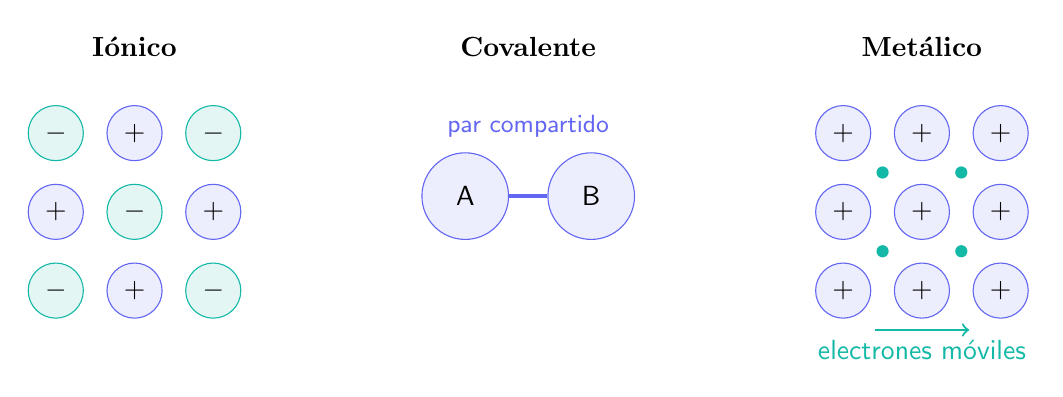
\begin{tikzpicture}[font=\sffamily]
  \node[font=\bfseries] at (0,3.1) {I\'onico};
  \foreach \x in {-1,0,1} \foreach \y in {0,1,2} {
    \pgfmathtruncatemacro{\s}{mod(\x+\y+10,2)}
    \ifnum\s=0 \node[circle,draw=nebula,fill=nebula!12,minimum size=7mm] at (\x,\y) {$+$};
    \else \node[circle,draw=spark,fill=spark!12,minimum size=7mm] at (\x,\y) {$-$};\fi}
  \node[font=\bfseries] at (5,3.1) {Covalente};
  \node[circle,draw=nebula,fill=nebula!12,minimum size=11mm] (a) at (4.2,1.2) {A};
  \node[circle,draw=nebula,fill=nebula!12,minimum size=11mm] (b) at (5.8,1.2) {B};
  \draw[very thick,nebula] (a)--(b);
  \node[text=nebula,anchor=south] at (5,1.82) {\small par compartido};
  \node[font=\bfseries] at (10,3.1) {Met\'alico};
  \foreach \x in {9,10,11} \foreach \y in {0,1,2} \node[circle,draw=nebula,fill=nebula!12,minimum size=7mm] at (\x,\y) {$+$};
  \foreach \p in {(9.5,.5),(10.5,.5),(9.5,1.5),(10.5,1.5)} \fill[spark] \p circle (2.2pt);
  \draw[->,spark,thick] (9.4,-.5)--(10.6,-.5) node[midway,below] {electrones m\'oviles};
\end{tikzpicture}
\end{document}
